\documentclass[11pt]{article}

% Packages for math. MUST LOAD BEFORE FONT PACKAGES
\usepackage{amsmath, amssymb, amsthm}


% Set font to Palatino
\usepackage{newpxmath}
\usepackage{newpxtext}
\linespread{1.05}         % Palatino needs more leading (space between lines)
\usepackage[T1]{fontenc}

\usepackage{microtype}
\usepackage{url}
\usepackage{tikz}
\usetikzlibrary{patterns}

\usepackage{color}
\usepackage{tcolorbox}



\usepackage[colorlinks=true,urlcolor=blue,linkcolor=blue]{hyperref}


% Page margins
\usepackage[margin=1in]{geometry}


% Theorem environments
\newtheorem{theorem}{Theorem}
\newtheorem{lemma}[theorem]{Lemma}
\newtheorem{proposition}[theorem]{Proposition}
\newtheorem{corollary}[theorem]{Corollary}
\newtheorem{fact}[theorem]{Fact}
\newtheorem{definition}[theorem]{Definition}
\newtheorem{example}[theorem]{Example}
\newtheorem{remark}[theorem]{Remark}
\newtheorem{problem}[theorem]{Problem}
\newtheorem*{question}{Question}
\newtheorem{exercise}[theorem]{Exercise}

% Delimiter macros
\newcommand{\paren}[1]{\left( #1 \right)}
\newcommand{\brac}[1]{\left[ #1 \right]}
\newcommand{\iprod}[1]{\langle #1 \rangle}
\newcommand{\abs}[1]{\left| #1 \right|}
\newcommand{\norm}[1]{\left\| #1 \right\|}

% Macros for real and natural numbers
\newcommand{\R}{\mathbb{R}} % Real numbers
\newcommand{\N}{\mathbb{N}} % Natural numbers

\renewcommand{\epsilon}{\varepsilon}
\newcommand{\eps}{\epsilon}

% Alphabet
\newcommand{\cA}{\mathcal{A}}
\newcommand{\cC}{\mathcal{C}}
\newcommand{\cL}{\mathcal{L}}
\newcommand{\cN}{\mathcal{N}}
\newcommand{\cQ}{\mathcal{Q}}


% Macros for probability
\DeclareMathOperator{\E}{\mathbb{E}} % Expectation
\DeclareMathOperator{\pE}{\widetilde{\mathbb{E}}} % Pseudoexpectation
\DeclareMathOperator{\Tr}{Tr} % Pseudoexpectation


% Macros for optimization
\newcommand{\OPT}{\text{OPT}}
\newcommand{\SoS}{\text{SoS}}

% Macro for indicator function
\newcommand{\Ind}[1]{\mathbf{1}\left ( #1\right )}

% Title and author information
\title{Lectures 1-4: Quadratic Proofs  and Max-Cut}
\author{Samuel B. Hopkins}
\date{\today}

% Document starts here
\begin{document}

\maketitle

\begin{figure}[h]
  \begin{center}
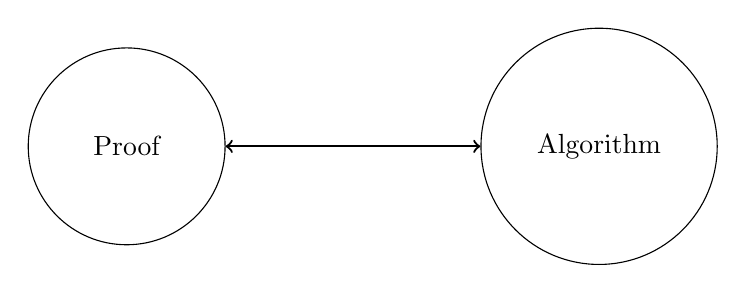
\begin{tikzpicture}
  % Draw the first bubble with text "proof"
  \node[draw, circle, minimum width=2.5cm, minimum height=1.5cm] (proof) at (0,0) {Proof};
  
  % Draw the second bubble with text "algorithm"
  \node[draw, circle, minimum width=3cm, minimum height=1.5cm] (algorithm) at (6,0) {Algorithm};
  
  % Draw arrows going back and forth between the bubbles
  \draw[<->, thick] (proof) -- (algorithm);
  
\end{tikzpicture}
\end{center}
\caption{This course in a nutshell.}
\end{figure}

\noindent \emph{Reader beware: these notes have not been subjected to the usual scrutiny reserved for peer-reviewed publication, and may contain errors.}

\vspace{1em}

This course is about a perspective on algorithm design which has come to be known as the \emph{sum of squares method}, or \emph{SoS} for short.
SoS originated in control theory and optimization, but has found a new home in theoretical computer science.
SoS has been key to numerous recent algorithmic innovations in TCS, including algorithms for graph partitioning, high-dimensional statistics, learning theory, quantum information, cryptography/cryptoanalysis, and beyond.

At the end of this course, you should have the ability to understand the increasingly-broad research literature in TCS in which SoS is used, and to apply SoS to new problems in your own research.

It is traditional to start a course like this by discussing one of the first major application of SoS in TCS: the Goemans-Williamson approximation algorithm for the maximum cut problem.
Often this algorithm is presented in a somewhat mysterious way, without much connection to algorithmic concepts which would be familiar from an undergraduate algorithms course.
I will opt for a slower presentation, with the goal of arriving at the Goemans-Williamson algorithm as an almost-inevitable consequence of applying general principles from the SoS method to the maximum cut problem.
This, of course, also gives us the opportunity to introduce those principles.

\section{Minimum and Maximum Cuts}

Let's start with the minimum and maximum cut problems.
\begin{problem}[Min-$(s,t)$-Cut]
Given a graph $G = (V,E)$ and $s,t \in V$, find $S \subseteq V$ such that $s \in S$ and $t \in \overline{S}$ minimizing the number of cut edges $E(S,\overline{S})$.
\end{problem}

Min-cut can be solved in polynomial time, e.g. by using Ford-Fulkerson or another max-flow algorithm to find the maximum flow in the graph from $s,t$, then finding all the vertices reachable from $s$ in this flow's residual graph.

\begin{problem}[Max-Cut]
Given a graph $G = (V,E)$, find $S \subseteq V$ maximizing the number of cut edges $E(S,\overline{S})$.
\end{problem}

Unlike its friend Min-Cut, Max-Cut is NP-hard, so we do not expect to design a polynomial-time algorithm for it.
Instead, we will aim for an \emph{approximation algorithm}.
As a reminder, an $\alpha$-approximation algorithm ($\alpha \geq 1$) for Max-Cut takes a graph $G$ and outputs a cut $S \subseteq V$ such that $E(S,\overline{S}) \geq \frac 1 \alpha \cdot \text{OPT}$, where $\text{OPT}$ is the number of cut edges in the optimal solution.

\paragraph{$2$-approximation for Max-Cut}
The simplest approximation algorithm for Max-Cut is the following: include each $v \in V$ in $S$ independently with probability $1/2$.

It is easy to show that every edge $(i,j)$ is cut with probability $1/2$, so the expected number of cut edges is $|E|/2$.
At the same time, the optimum value $\text{OPT} \leq |E|$ -- we can't do better than cutting all of the edges.
So
\[
\E_S E(S,\overline{S}) = \frac{|E|}{2} \geq \frac{\text{OPT}}{2} \, ,
\]
and hence the algorithm is a $2$-approximation.
As an aside, this algorithm can be derandomized into a greedy algorithm.

\begin{question}
Can we do better than a $2$-approximation for Max-Cut?
\end{question}

\noindent To investigate, we will take a detour to the world of \emph{proofs} and \emph{proof systems}.

\section{Proofs and (Approximation) Algorithms}
\begin{quote}
    \begin{center}
\emph{Every approximation algorithm is a proof system for proving bounds on \text{OPT}.}
    \end{center}
\end{quote}
Let us explain what is meant by this sentence in the contexts of Min-Cut and Max-Cut, staying informal for now about what we mean by a ``proof system.'' 

\subsection{Min-Cut}
\paragraph{Upper bounds on Min-Cut} Suppose $G$ is a graph held by a prover, Alice, who claims that $\text{Min-Cut(G)} \leq k$.
Alice can convince a polynomial-time verifier, Bob, of this fact, by supplying him with a cut $S \subseteq V$ such that $E(S,\overline{S}) \leq k$.
Given the cut $S$, Bob can verify that $E(S,\overline{S}) \leq k$ in polynomial time. This is the argument which shows Min-Cut is in NP.

\paragraph{Lower bounds on Min-Cut} What if Alice claims that $\text{Min-Cut(G)} \geq k$? What kind of proof could she show Bob? 
As you might recall from undegraduate algorithms, one type of proof Alice could use is a valid flow from $s$ to $t$.
If Alice can show Bob a flow of value $k$ from $s$ to $t$, meaning that she tells Bob how much flow to route on each edge of $G$, Bob can easily check that the flow is valid and that its value is $k$, and hence that $\text{Min-Cut}(G) \geq k$.

The max-flow min-cut theorem says that this kind of proof actually always exists -- there is always an $(s,t)$ flow of value $\text{Min-Cut}(G)$, and hence Alice can always convince Bob of any true statement of the form $\text{Min-Cut}(G) \geq k$ by showing him a flow of value $k$.

\subsection{Max-Cut}
\paragraph{Lower bounds on Max-Cut} Similar to the case of upper bounds on the Min-Cut, suppose Alice claims that $\text{Max-Cut}(G) \geq k$.
Alice can convince a polynomial-time verifier, Bob, of this fact, by simply supplying him with a cut $S \subseteq V$ such that $E(S,\overline{S}) \geq k$.

\paragraph{Upper bounds on $\OPT$} But now what if Alice claims that $\OPT \leq k$?
What kind of proof could she show Bob to convince him of this fact?
Not so clear!

\subsection{Approximation Algorithms are Proof Systems}
Before we turn to particular kinds of proofs Alice might use, let's justify the point of this detour: if there is a (deterministic) $\alpha$-approximation algorithm ALG for Max-Cut, then there is a way for Alice to convince Bob that $\OPT \leq \alpha \cdot k$ whenever $\OPT \leq k$.\footnote{Or, in complexity-theoretic terms, $P \subseteq NP \cap coNP$.}

One way would be for Bob to just run ALG -- whatever cut $S$ ALG outputs will have value $E(S,\overline{S}) \leq \OPT \leq k$, and since ALG is an $\alpha$-approximation algorithm, seeing ALG output $S$ will convince Bob that $\OPT \leq \alpha E(S,\overline{S}) \leq \alpha k$.

If we want to be more explicit about the proof system, we can imagine that Alice sends Bob a transcript of the execution of ALG, and Bob can verify that the transcript is correct and that the cut $S$ output by ALG has value at most $k$, and hence that $\OPT \leq \alpha k$.

So, if we design, say, a $1.99$-approximation algorithm for Max-Cut, in the course of doing so we will have implicitly designed a proof system which Alice could use to convince Bob that $\OPT \leq 1.99 k$ whenever $\OPT \leq k$.
We might as well try to design the proof system explicitly.

\section{Linear Proofs}
Our goal is to design a proof system which Alice can use to convince Bob that $\text{Max-Cut}(G) \leq k$.
To get inspiration, let's return to Min-Cut and have a more explicit look at the proof system for lower bounds on Min-Cut, through the lens of linear programming.

\subsection{Linear Proofs and Min-Cut}
We'll start by writing down a linear program for Min-$(s,t)$-Cut.
Our LP will have variables $x_v$ for $v \in V$, and also $y_{uv}$ for edges $(u,v) \in E$.
The intended meaning of the variables will be that $x_v = 1$ if $v \in S$ and $x_v = 0$ otherwise, and $y_{uv} = 1$ if $(u,v)$ is a cut edge and $y_{uv} = 0$ otherwise.
The LP is:
\begin{align}
\min_{x,y} & \sum_{(u,v) \in E} y_{uv} \, \, \text{ such that } \\
& x_s = 1 \\
& x_t = 0 \\
& 0 \leq y_{uv} \, \forall (u,v) \in E\\
& y_{uv} \geq x_u - x_v  \, \, \forall (u,v) \in E \, .
\end{align}
We are taking the tuples $(u,v)$ to be ordered, and when there is an edge between $u$ and $v$ we assume $E$ contains $(u,v)$ and $(v,u)$.
Notice that the final set of constraints encode the fact that $y_{uv} = 1$ only if $(u,v)$ is a cut edge with $x_u = 1$ and $x_v = 0$.
We won't prove it, but this LP is actually tight: the optimal value is exactly equal to the Min-$(s,t)$-Cut value.

The LP offers a proof system for proving lower bounds on the Min-$(s,t)$-Cut value via duality.
As a reminder, a dual solution to the above LP consists of numbers $\lambda_s, \lambda_t \in \R$ (multipliers for the constraints $x_s = 1, x_t = 0$) and $\alpha_{u,v}, f_{uv} \geq 0$ for $(u,v) \in E$ (multipliers for the inequality constraints) such that
\[
  \sum_{(u,v) \in E} y_{uv} - k = \lambda_s(x_s-1) + \lambda_t x_t + \sum_{(u,v) \in E} \alpha_{uv} y_{uv} + f_{uv}(y_{uv} - (x_u - x_v)) \, 
\]
where here we mean equality \emph{as linear functions of $x$ and $y$}.
Because the RHS of the inequality above must be nonnegative for every feasible solution $x,y$, the LHS must be as well, meaning that the Min-$(s,t)$-Cut value is at least $k$.
If Alice shows Bob the dual solution, he can verify that it satisfies the above equality by checking that the coefficient of each variable $x_i$ is the same on both sides.

This LP-based proof system is actually \emph{equivalent} to the max-flow proof system from above!
It's not too hard to prove that in order to satisfy the above equality, the dual variables $f_{uv}$ have to be a valid $t,s$ flow of value $k$, where we route $f_{uv}$ units of flow from $u$ to $v$.
\begin{proof}[Proof sketch that $f_{uv}$ is a valid flow of value $k$]
    The coefficient of $y_{uv}$ on the RHS is $\alpha_{uv} + f_{uv}$ and on the LHS it's $1$.
    So we must have $1 = \alpha_{uv} + f_{uv}$, and hence $f_{uv} \in [0,1]$.
    Thus $f$ respects the edge capacities.
    
    For $v \neq s,t$, the coefficient of $x_v$ on the RHS is $\sum_{u \in N(v)} f_{uv} - f_{vu}$, and on the LHS it's $0$.
    So we must have $\sum_{u \in N(v)} f_{uv} = \sum_{u \in N(v)} f_{vu}$ -- that is, the incoming flow equals the outgoing flow at vertex $v$.

    The constant term on the RHS is $-\lambda_s$ and on the LHS it's $-k$, so we must have $\lambda_s = k$.
    But, the coefficient of $x_s$ on the RHS is $\lambda_s + \sum_{u \in N(s)} f_{sv} - f_{vs}$ and on the LHS it's $0$.
    So we must have $\sum_{u \in N(s)} f_{sv} - f_{vs} = -k$, meaning that $k$ units of flow are routed into $s$.
\end{proof}

Furthermore, reformulating what we said before about the max-flow proof system, by the max-flow min-cut theorem, whenever $\text{Min-Cut}(G) \geq k$, Alice can prove this to Bob by exhibiting such $\lambda, \alpha,$ and $f$.

\subsection{Linear Proofs and Max-Cut}
A linear proof system turned out to be as powerful as we could hope for for Min-Cut.
How about for Max-Cut?
Of course we don't expect to come up with an exact LP formulation of Max-Cut, but perhaps we can arrive at a useful LP relaxation and a corresponding proof system nonetheless.
(Even more optimistically, we might then hope to use that LP to go beyond a proof system and actually design an approximation algorithm.)

Unfortunately, this approach won't work out -- in fact, one can show that there is no polynomial-size LP relaxation of Max-Cut which gives a $2-\eps$ approximation for any $\eps > 0$ (although that result is beyond the scope of this class).
But let's try to see why we can't just use the same type of LP as for Min-Cut.

As for Min-Cut, we can have variables $x_v$ for $v \in V$ and $y_{uv}$ for $(u,v) \in E$, with the intended meanings that $y_{uv} = 1$ if $(u,v)$ is a cut edge and $y_{uv} = 0$ otherwise, and $x_u = 1$ if $u \in S$ and $x_u = 0$ otherwise.
The objective function is easy enough to write: $\max \sum_{(u,v) \in E} y_{uv}$.
But how can we constrain $y_{uv}$ so that it is $1$ only if $(u,v)$ is a cut edge?
In the Min-Cut case used the fact that the LP was trying to minimize $y_{uv}$, together with the constraints $y_{uv} \geq x_u - x_v$, to force $y_{uv}$ to act like the indicator for a cut edge.
Now the LP is trying to maximize $y_{uv}$, so we can't use the same trick.

Of course, we could write down a silly LP relaxation of Max-Cut:
\[
  \max_{y} \sum_{(u,v) \in E} y_{uv} \text{ s.t. } 0 \leq y_{uv} \leq 1 \, .
\]
(Now we think of the $(u,v)$ pairs as un-ordered.)
The optimum value will always by $|E|$, meaning that this LP gives just a $2$-approximation to the value of the Max-Cut.
Just for fun, let's see the proof system that this LP gives us: there are dual variables $\alpha_{uv}, \lambda_{uv} \geq 0$, and to prove that $\text{Max-Cut}(G) \leq k$ we require that
\[
k - \sum_{(u,v) \in E} y_{uv} = \sum_{(u,v) \in E} \alpha_{uv} y_{uv} + \lambda_{uv}(1- y_{uv}) \, .
\]
Unfortunately, this linear proof system for Max-Cut will never let Alice prove anything better than $\text{Max-Cut}(G) \leq |E|$.

\section{Quadratic Proofs}
The linear proof system for Max-Cut was not very useful.
Our LP relaxation didn't work well because we didn't have a good way to express the constraint that $y_{uv} = 1$ only if $(u,v)$ is a cut edge.

Observe, however, that if we were not so tied to linear functions of our variables, we would not have this issue.
It is traditional at this point to switch to placing the $x_v$ variables in $\{-1,1\}$.
For $x_u,x_v \in \{-1,1\}$ we could directly write the indicator $\Ind{x_u \neq x_v}$ as a quadratic function of $x_u, x_v$:

\[
\Ind{x_u \neq x_v} = \frac 12 (1 - x_u x_v)
\]
so that the Max-Cut objective function would be
\[
  \max_x \, \frac 12 \sum_{(u,v) \in E} \frac 12 - \frac{x_u x_v}{2} \, .
\]

Now let's see how we could use this quadratic objective function to define a proof system for Max-Cut.
Suppose, as usual, that Alice wants to prove to Bob that $\text{Max-Cut}(G) \leq k$.
In the linear proofs setting, Alice showed Bob a way to write the difference of $k$ and the (linear) objective function as a sum of pieces which Bob could easily verify were nonnegative.
The ``pieces'' were linear functions induced by constraints from the LP, which Bob knows must be nonnegative for any feasible solution $y$.
It is important that Bob has such an \emph{a priori} reason to believe that the pieces are nonnegative, because he does not have time to check nonnegativity for every feasible $y$.

Now the objective function is quadratic in $x$.
What are some \emph{quadratic} functions of $x$ that Bob can easily check are nonnegative for any feasible solution $x$?

\begin{quote}
\begin{center}
\emph{\textbf{Big idea:} The square of every linear function with real coefficients is everywhere nonnegative!}
\end{center}
\end{quote}

So, suppose Alice could find $m$ linear functions $f_1(x),\ldots,f_m(x)$ -- that is, each $f_i$ has the form
\[
f_i(x) = \sum_{v \in V} f_{iv} x_v
\]
where $f_{iv} \in \R$ -- such that for every $x \in \{-1,1\}^V$,
\[
  k - \sum_{(u,v) \in E} \frac 12  - \frac{x_u x_v}{2} = \sum_{i=1}^m f_i(x)^2 \, .
\]
Then, assuming that Bob could actually check that this equation holds for all $x \in \{-1,1\}^V$, he would be convinced that $\text{Max-Cut}(G) \leq k$.

How could Bob convince himself that the equation holds for all $x \in \{-1,1\}^V$, without spending time $2^{|V|}$?
If Bob were trying to verify that the equation holds for every $x \in \R^{V}$, he could just check that the coefficient of every degree-$2$ monomial $x_u x_v$ on the LHS is equal to the coefficient of the same monomial on the RHS.
It turns out that a similar approach works for $x \in \{-1,1\}^V$, because of the multivariate discrete Fourier transform:
\begin{fact}
  Every function $f: \{-1,1\}^n \to \R$ can be written uniquely as a multilinear polynomial in the $x_i$'s; that is, $f(x) = \sum_{S \subseteq [n]} \hat{f}_S \cdot \prod_{i \in S} x_i$ where $\hat{f}_S \in \R$.
\end{fact}
So, given $f_1,\ldots,f_m$, Bob can expand $\sum_{i=1}^m f_i(x)^2$ in the monomial basis and replace each non-multilinear term $x_v^2$ with $1$.
Then he can compare the coefficients of each monomial on the LHS and RHS to verify that the equation holds for all $x \in \{-1,1\}^V$.
This verification procedure clearly runs in time polynomial in $|V|,m$.

We are left with (at least) three questions:

\begin{enumerate}
    \item (Proof existence) For which $k$ can Alice find a proof that $\text{Max-Cut}(G) \leq k$? In particular, do such proofs exist for $k < |E|$?
    \item (Proof size) How many linear functions $f_1,\ldots,f_m$ does Alice need to prove that $\text{Max-Cut}(G) \leq k$?
    In particular, can we always assume that the proof is polynomial-size, i.e. $m \leq |V|^{O(1)}$?
    (And, more subtly, that each $f_i$ has bit complexity $|V|^{O(1)}$?)
    \item (Algorithm) Do quadratic proofs like this correspond to a useful polynomial-time algorithm?
\end{enumerate}

Before we answer these questions, we'll do some examples to gain a bit of intuition about quadratic proofs.

\subsection{Quadratic proofs at least as good as linear ones}
To make sure we haven't accidentally made our lives worse, we should make sure that we can find a quadratic proof that $\text{Max-Cut}(G) \leq |E|$.
In other words, can we find a sum-of-squares representation of the function 
\[
|E| - \sum_{(u,v) \in E} \frac 12 - \frac{x_u x_v}{2}  = \frac {|E|}{2} + \sum_{(u,v) \in E} \frac{x_u x_v}{2}\, ?
\]
We can do this by observing that $(x_u + x_v)^2 = x_u^2 + x_v^2 + 2 x_u x_v = 2 + 2 x_u x_v$, so
\[
\frac {|E|}{2} + \sum_{(u,v) \in E} \frac{x_u x_v}{2} = \sum_{(u,v) \in E} \frac 14 (x_u + x_v)^2 \, .
\]

\subsection{Quadratic proofs can be better than linear ones: the triangle}
The simplest graph $G = (V,E)$ whose maximum cut is strictly smaller than $|E|$ is the triangle. 
(Every one and two edge graph is bipartite.)
So, let $V = \{1,2,3\}$ and edges $E = \{(1,2),(2,3),(3,1)\}$:
\[
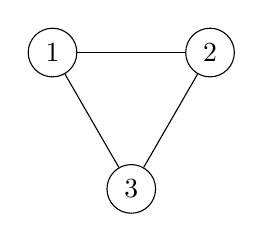
\begin{tikzpicture}
    \node[circle, draw] (1) at (0,0) {1};
    \node[circle, draw] (2) at (2,0) {2};
    \node[circle, draw] (3) at (1,-1.732) {3};
    
    \draw (1) -- (2);
    \draw (2) -- (3);
    \draw (3) -- (1);
\end{tikzpicture}
\]

The actual Max-Cut value is $2$.
The best upper bound we could hope for from a linear proof system is $|E| = 3$.
Can we find a quadratic proof that $\text{Max-Cut}(G) \leq 2.9 < 3$?
In fact, there's a simple way to do so: note that
\[
  (x_1 + x_2 + x_3)^2 = x_1^2 + x_2^2 + x_3^2 + 2(x_1 x_2 + x_2 x_3 + x_3 x_1) = 3 + 2(x_1 x_2 + x_2 x_3 + x_3 x_1) \, .
\]
So,
\[
  2.25 - (\frac 12 - \frac{x_1 x_2}{2}) - (\frac 12 -\frac{x_2 x_3}{2}) - (\frac 12 - \frac{x_3 x_1}{2}) = \frac 14 (x_1 + x_2 + x_3)^2 \, .
\]
This is our first proof which beats the linear proof system!

\subsection{Quadratic proofs from eigenvalues}
The triangle graph is pretty simple.
It actually turns out that quadratic proofs improve over linear proofs for \emph{every} non-bipartite graph.
(For a bipartite graph the maximum cut value is actually $|E|$.)
For simplicity, we will illustrate this only for regular graphs.

\begin{fact}
\label{fact:non-bipartite-eigenvalues}
Let $A$ be the adjacency matrix of a connected, $d$-regular non-bipartite graph $G = (V,E)$.
Then the least eigenvalue $\lambda_{\min}(A)$ satisfies $\lambda_{\min}(A) > -d$.
\end{fact}
\begin{proof}
  Suppose for contradiction that $v$ is an eigenvector of $A$ with eigenvalue $-d$; let $\|v\| = 1$
  Then $v$ would be orthogonal to the all-$1$s vector, so it has some negative and some positive coordinates.
  Now consider $(Av)_i = \sum_{j \sim i} v_j$, and hence
  \[
  d^2 \|v\|^2 = \|Av\|^2 = \sum_{i} \paren{\sum_{j \sim i} v_j}^2 \, .
  \]
  Now, by Cauchy-Schwarz, each term $(\sum_{j \sim i} v_j)^2 \leq d \sum_{j \sim i} v_j^2$, with equality only if $v_j = v_k$ for all $j,k \sim i$.
  But indeed the equality case must obtain for all $i$, since $\sum_{i} \paren{\sum_{j \sim i} v_j}^2 = d^2 \|v\|^2$.
  
  We claim that the partition of $V$ into vertices $i$ for which $v_i \leq 0$ and $v_i > 0$ is a bipartition of $G$.
  Suppose for a contradiction that there is an edge $i \sim j$ for a pair $i,j$ with $v_i,v_j > 0$.
  Then every neighbor of $i$ must have $v_k > 0$, and similarly for $j$ -- iterating this argument, $v$ must be nonnegative on the entire connected component containing $i$ and $j$ -- since $G$ is connected, this is all of $V$.
  But that's a contradiction, since $v$ is orthogonal to the all-$1$s vector.
\end{proof}

It turns out that the fact that $\lambda_{\min}(A) > -d$ is enough to give a quadratic proof that $\text{Max-Cut}(G) < |E|$.

\begin{theorem}
  \label{thm:eigenvalue-proof}
  Fix a $d$-regular graph $G = (V,E)$ with adjacency matrix $A$.
  There is a quadratic proof that $\text{Max-Cut}(G) \leq \tfrac 12 (1 - \tfrac{\lambda_{\min}(A)}{d}) |E|$
\end{theorem}
To prove Theorem~\ref{thm:eigenvalue-proof}, we need a linear algebra refresher.
\begin{tcolorbox}[colback=white, colframe=black, width=\textwidth, boxrule=0.5mm]
\textbf{Positive-Semidefinite Matrices:}
For a symmetric matrix $M \in \R^{n \times n}$, the following are equivalent.
If $M$ satisfies any/all of them, we say it is \emph{positive semi-definite}, or \emph{PSD}.
\begin{enumerate}
  \item $M$ has all nonnegative eigenvalues.
  \item For all $x \in \R^n$, $\iprod{x, Mx} \geq 0$.
  \item There is a matrix $L \in \R^{n \times n}$ such that $M = L L^\top$.
\end{enumerate}
\end{tcolorbox}

We need a lemma to relate eigenvalues to quadratic proofs:
\begin{lemma}
\label{lem:operator-norm}
Let $M \in \R^{n \times n}$ be a symmetric matrix.
There exist $n$ linear functions $f_1,\ldots,f_n$ on $n$ variables such that \[ |\lambda_{\min}(M)| \cdot \|x\|^2 + x^\top M x = \sum_{i=1}^n f_i(x)^2 \, .\]
(Here the equality holds as degree-2 polynomials over $\R^n$.)
\end{lemma}
\begin{proof}[Proof of Lemma~\ref{lem:operator-norm}]
    The matrix $|\lambda_{\min}(M)| \cdot I + M$ is positive semi-definite (where $I$ is the identity matrix), so it has a decomposition as $LL^\top$.
    Take $f_i(x) = \sum_{j=1}^n L_{ij} x_j$.
\end{proof}

Now we can prove Theorem~\ref{thm:eigenvalue-proof}.

\begin{proof}[Proof of Theorem~\ref{thm:eigenvalue-proof}]
    We can write the Max-Cut objective function as
    \[\sum_{(i,j) \in E} \frac 12 - \frac{x_i x_j}{2} = \frac{|E|}{2} - \frac 14 x^\top A x = \frac{|E|}{2} + \frac 14 x^\top \paren{\lambda_{\min}(A) \cdot I - A} x - \frac 14 \lambda_{\min}(A) \cdot \|x\|^2 \, ,\]
    where the $1/4$ shows up because each edge appears twice in $x^\top A x$, as $A$ is a symmetric matrix.
    Now we can apply Theorem~\ref{thm:eigenvalue-proof} to conclude that there is a degree-2 sos polynomial $SoS(x)$ such that
    \[
    \text{Max-Cut}(G) = \frac{|E|}{2} + SoS(x) - \frac 14 \lambda_{\min}(A) \cdot \|x\|^2 \, .
    \]
    Now, for every $x \in \{ \pm 1\}^n$, we have $\|x\|^2 = n = 2 |E| / d$.
    So for every $x \in \{ \pm 1\}^n$, we have
    \[
    \frac{|E|}{2} + SoS(x) - \frac 14 \lambda_{\min}(A) \cdot \|x\|^2 = \frac 12 \paren{1 - \frac{\lambda_{\min}(A)}{d}} |E| \, ,
    \]
    which concludes the proof.
\end{proof}

It turns out that this eigenvalue-based SoS proof is enough to show a strong result for random graphs, although we won't be equipped to prove this until later in the semester when we get acquainted with random matrices.

\begin{theorem}
\label{thm:random-graph}
With high probability over the choice of $G \sim G(n,1/2)$, there is a polynomial-size quadratic proof that $\text{Max-Cut}(G) \leq (0.5 + o(1)) |E|$.
\end{theorem}


\section{From Quadratic Proofs to an Algorithm for Max-Cut}
We have a promising proof system on our hands.
How could we use it to design an (approximation) algorithm for Max-Cut?

\subsection{Convexity, Duality and Pseudoexpectations}
In the Min-Cut setting, where we had a linear proof system, the proof system and the Min-Cut LP were related by LP duality.
We would like to find an appropriate generalization of LP duality which will enable us to convert our quadratic proof system into an approximation algorithm for Max-Cut.
As a first step, we observe that the set of ``possible right-hand sides'' for a quadratic proof is convex.

\begin{lemma}[Convexity of Sum-of-Squares Polynomials]
  For any $d \in \N$, the set of functions $p(x) \, : \, \{-1,1\}^n \rightarrow \R$ for which there exist $f_1,\ldots,f_m$ of degree $\leq d$ such that $p(x) = \sum_{i=1}^m f_i(x)^2$ for all $x \in \{-1,1\}^n$ is convex.
  We call this set $\SoS_d$
\end{lemma}
\begin{proof}
The proof is straightforward: if $p(x) = \sum_{i=1}^m f_i(x)^2$ and $q(x) = \sum_{i=1}^m g_i(x)^2$, then for any $\lambda \in [0,1]$ we have
\[
  \lambda p(x) + (1-\lambda) q(x) = \sum_{i=1}^m (\sqrt{\lambda} f_i(x))^2 + ( \sqrt{(1-\lambda)} g_i(x))^2 \, . \qedhere
\]
\end{proof}

So we can phrase the question ``is there a quadratic proof that $\text{Max-Cut}(G) \leq k$?'' as a convex membership problem: is $k - \sum_{(i,j) \in E} \frac 12 - \frac{x_i x_j}{2}$ in $\SoS_1$?



\begin{tcolorbox}[colback=white, colframe=black, width=\textwidth, boxrule=0.5mm]
\textbf{Convex Duality 101 (Informal):}
Recall that $\cC \subseteq \R^n$ is convex if for every $x,y \in \cC$, also $\tfrac{x+y}{2} \in \cC$.
There is a rich theory of convex geometry -- we will discuss a tiny portion of it, on the topic of 
convex duality, and not be particularly formal about it for now.
Formal treatments, handling technical issues I won't discuss here, are available in many textbooks.

\vspace{0.5em}

Every convex $\cC$ set looks kind of like this:

\begin{center}
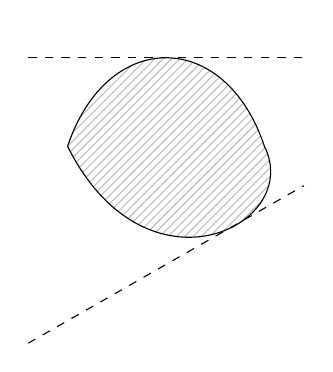
\begin{tikzpicture}

% Draw the convex set
\filldraw[pattern=north east lines, pattern color=gray!50] 
    (0,0) .. controls (0.5,1.5) and (2,1.5) .. (2.5,0) 
    .. controls (3,-1) and (1,-2) .. (0,0);

% Supporting hyperplane 1
\draw[dashed] (-0.5,1.13) -- (3,1.13);

% Supporting hyperplane 3
\draw[dashed] (-0.5,-2.5) -- (3,-0.5);

\end{tikzpicture}

\end{center}

The dashed lines are ``supporting hyperplanes''  of $\cC$ -- they are hyperplanes which lie on one side of $\cC$, and intersect (the closure of) $\cC$ at one or more points.
Every point on the boundary of a convex set is intersected by some supporting hyperplane. 
A ``separating'' hyperplane lies on one side of the convex set, and need not intersect $\cC$ at any point.
The set of all separating hyperplanes is called the ``dual'' of $\cC$.

\vspace{0.5em}

Formally, if $\cC \subseteq \R^n$ is a convex set, a separating hyperplane is an affine function $f \, : \, \R^n \rightarrow \R$ such that $f(x) \geq 0$ for all $x \in C$.
The hyperplane $f$ is supporting if there is some $x$ in the closure of $\cC$ with $f(x) = 0$.
Convexity of the set of separating hyperplanes is clear: if $f(x), g(x) \geq 0$ for all $x \in \cC$, then also $\tfrac{f(x) + g(x)}{2} \geq 0$.

\vspace{0.5em}

Furthermore, any $x \notin \text{closure}(\cC)$ if and only if there is a separating hyperplane for $x$; that is a separating hyperplane $f$ of $\cC$ such that $f(x) < 0$.
\end{tcolorbox}

\paragraph{Duals to Quadratic Proofs}
Now that we know about convex duality, let's figure out what the convex dual of $\SoS_1$ is.
Let us think of $\SoS_1$ as a subset of $\R[x_1,\ldots,x_n]_{\leq 2}^m$, the vector space of multilinear polynomials in variables $x_1,\ldots,x_n$ with real coefficients and degree at most $2$.\footnote{If we want to be picky about thinking of convex sets as living in $\R^N$ for some value of $N$, we could identify $\R[x_1,\ldots,x_n]_{\leq 2}$ with $\R^{\binom{N}{2} + N + 1}$ by identifying a polynomial with the list its of coefficients in the monomial basis.}
(The ``$m$'' stands for multilinear -- it is not standard notation.)
A separating hyperplane for $\SoS_1$ is an affine function $\cL \, : \,  \rightarrow \R$ such that $\cL[p] \geq 0$ for all $p \in \SoS_1$.\footnote{We use the notation $\cL[p]$ for the function $\cL$ applied to the polynomial $p$, rather than $\cL(p)$, for reasons which will be clear later.}
Because of some special structure of $\SoS_1$ (it is actually a convex \emph{cone}), we'll be able to assume that $\cL$ is actually linear rather than affine, and satisfies a normalization condition.
This is captured by the following theorem.
\begin{theorem}
  \label{thm:duality}
  Let $p \in \R[x_1,\ldots,x_n]_{\leq 2}^m$ and let $\eps > 0$.
  If $p + \epsilon \notin \SoS_1$, then there is a linear function $\pE \, : \, \R[x_1,\ldots,x_n]_{\leq 2}^m \rightarrow \R$ satisfying:
  \begin{enumerate}
  \item Positivity on SoS polynomials: $\pE[q(x)] \geq 0$ for every $q \in \SoS_1$
  \item Normalization: $\pE[1] = 1$
  \item Separation: $\pE[p(x)] < 0$.
  \end{enumerate}
  Conversely, if such a $\pE$ exists, then $p \notin \SoS_1$.
\end{theorem}
\begin{proof}
  The ``if'' direction is clear, so we prove the ``only if''.
  By the separating hyperplane theorem for convex sets, $p + \eps \notin \SoS_1$ implies that there is a hyperplane $\cL$ separating $p + \eps$ from $\SoS_1$.
  We claim that the linear function defined by $\cL'[q] = \cL[q] - \cL[0]$ for all $q$ also separates $p+\eps$ from $\SoS_1$.

  We claim that $\cL[0] \geq 0$, as otherwise there would be a positive $c > 0$ such that $\cL[c] < 0$, by continuity, but since $c = (\sqrt c)^2$ this can't happen.
  So, $\cL'[p + \eps] = \cL[p + \eps] - \cL[0] \leq 0$.

  It just remains to verify that $\cL'[q] \geq 0$ for every $q \in \SoS_1$; then we can scale $\cL'$ by a nonnegative scalar to make it satisfy the normalization condition.
  It will be enough to show that $\cL[q] \geq \cL[0]$ for every $q \in \SoS_1$.
  Fix $q \in \SoS_1$ and consider the affine function of a single real variable $\epsilon$ given by $t(\epsilon) = \cL[\epsilon q] = t_1 \epsilon + t_0$ for some real numbers $t_1, t_0$.
  We claim that $t_1 \geq 0$, as otherwise by taking $\epsilon$ sufficiently large, we could make $\cL[\epsilon q] < 0$, which is impossible.
  So, $t(\epsilon)$ is monotone decreasing in $\epsilon$.
  But $t(0) = \cL[0]$, so we are done.

  Let $\pE[q] = \cL[q] / \cL[1]$, so that $\pE[1] = 1$. 
  Then $\pE[p+\eps] \leq 0$, hence $\pE[p] < 0$.
\end{proof}

\begin{definition}[Pseudoexpectation over the Hypercube]
  We call a linear function $\pE \, : \, \R[x_1,\ldots,x_n]_{\leq 2}^m$ satisfying the positivity and normalization conditions of Theorem~\ref{thm:duality} a \emph{degree 2 pseudoexpectation}.
\end{definition}

We often extend a pseudoexpectation $\pE$ to a linear function on all of $\R[x_1,\ldots,x_n]_{\leq 2}$ by defining $\pE[x_i^2] = 1$ and extending linearly.
Notice that this extension has the property that two polynomials $p,q$ for which $p(x) = q(x)$ for all $x \in \{\pm 1\}^n$ must have $\pE[p(x)] = \pE[q(x)]$.
In particular, for every linear function $q(x)$, $\pE[q(x)^2] \geq 0$.


\paragraph{Duality for Max-Cut Quadratic Proofs}
Theorem~\ref{thm:duality} has the following consequence for Max-Cut:
\begin{corollary}
Let $G = (V,E)$ be a graph.
Then
\begin{align*}
  \inf \left \{ k \, : \,  k - \sum_{(i,j) \in E} \frac 12 - \frac{x_i x_j}{2}  \in \SoS_1 \right \} 
  = \sup \,  \pE \brac{ \sum_{(i,j) \in E} \frac 12 - \frac{x_i x_j}{2}} \, .
\end{align*}
\end{corollary}
\begin{proof}
  If $k$ is such that $k - \sum_{(i,j) \in E} \tfrac 12 - \tfrac{x_i x_j}{2} \notin \SoS_1$, then there exists $\pE$ such that
  \[
  \pE \brac{k - \eps - \sum_{(i,j) \in E} \frac 12 - \frac{x_i x_j}{2}} < 0 \, ,
  \]
  which rearranges to 
  \[
    \pE \brac{\sum_{(i,j) \in E} \frac 12 - \frac{x_i x_j}{2}} \geq \pE[k-\eps] = k -\eps \, . 
  \]
  Since this holds for every $\eps > 0$, we have the corollary.
\end{proof}

At this point, our hoped-for outline of an algorithm for Max-Cut is:
\begin{enumerate}
\item Given a graph $G$, find a pseudoexpectation $\pE$ maximizing $\pE[ \sum_{(i,j) \in E} \tfrac 12 - \tfrac{x_i x_j}{2}]$.
\item Use $\pE$ to find a cut in $G$ which cuts many edges.
\end{enumerate}

For (1), we can be optimistic, because the set of pseudoexpectations is convex and only $\approx n^2$-dimensional, when $G$ is an $n$-vertex graph, and we are trying to maximize a linear function over it.
The set of pseudoexpectations isn't a polytope (that is, the feasible region of a linear program), so we can't use linear programming for (1), but we will be able to use a generalization of linear programming called \emph{semidefinite programming}.
For now, we will pretend that we can solve (1) in polynomial time, and move on to (2), for which we need to understand better how to think of a pseudoexpectation.

\paragraph{What is a Pseudoexpectation, Anyway?}
We have a formal defintion of a pseudoexpectation, but it's not very intuitive.
A good way to think of a degree-$2$ pseudoexpectation is that is tells us the degree-two moments (that is, means and covariances) of a ``fictional'' probability distribution over $\{\pm 1\}^n$.

\begin{exercise}
Let $\mu$ be a probability distribution over $\{ \pm 1\}^n$ and define $\pE[p(x)] = \E_{x \sim \mu} p(x)$.
Show that $\pE$ is a degree-$2$ pseudoexpectation.
\end{exercise}

So, every distribution over the hypercube gives a pseudoexpectation.
The reverse is not true.

\begin{exercise}
Find a degree-2 pseudoexpectation $\pE$ over $\{ \pm 1\}^3$ which is not induced by any distribution over $\{ \pm 1\}^3$.
\end{exercise}

Even so, it helps to think of a pseudoexpectation as specifying moments of a probability distribution.
In the case of Max-Cut, the pseudoexpectation appears to be the second moments of a probability distribution over cuts in $G$ which cut a lot of edges.
Our goal is to use these second moments to find an actual cut which cuts a lot of edges.
It is tempting to try and sample from a distribution which induces the pseudoexpectation, but this isn't allowed -- there may be no such distribution!

To make things a little more concrete, let's see how we would represent a pseudoexpectation.
Recall that the monomials $1, x_1,\ldots,x_n,x_1 x_2, x_1 x_3,\ldots,x_{n-1}x_n$ form a basis for $\R[x_1,\ldots,x_n]_{\leq 2}^m$.
So we can specify $\pE$ by specifying $\pE x_1,\pE x_2,\ldots,\pE x_n, \pE x_1 x_2, \ldots$ for all multilinear monomials of degree $\leq 2$.
Any such list of $n + \binom{n}{2}$ numbers represents a linear operator from $\R[x_1,\ldots,x_n]_{\leq 2}$ to $\R$.
The following exercise shows that this list of numbers represents a pseudoexpectation if and only if an associated ``moment matrix'' is positive semi-definite.

\begin{exercise}
  Let $\pE$ be a linear operator from $\R[x_1,\ldots,x_n]_{\leq 2}$ to $\R$.
  Then $\pE$ satisfies the condition $\pE p^2 \geq 0$ for all $p$ with degree at most $1$ if and only if the matrix $\pE[(1,x)(1,x)^\top] \succeq 0$.
  Here the notation $(1,x)$ indicates the $(n+1)$-dimensional vector of degree $\leq 1$ monomials obtained by concatenating the constant function $1$ with the variables $x_1,\ldots,x_n$, so the matrix $\pE[(1,x)(1,x)^\top]$ contains the entries $\pE[1], \pE[x_1], \ldots, \pE[x_n], \pE[x_1^2] = 1, \pE[x_1 x_2] \ldots, \pE[x_n^2]=1$.
\end{exercise}




\subsection{Gaussian Rounding}
Goemans and Williamson had the following amazing idea for how to use a pseudoexpectation to find a cut which cuts a lot of edges.
To express it, we need the following lemma.
\begin{lemma}
Let $\pE$ be a degree-2 pseudoexpectation.
There is a Gaussian distribution $\cN$ over $\R^n$ such that for every $p \in \R[x_1,\ldots,x_n]_{\leq 2}^m$, we have $\pE[p(x)] = \E_{y \sim \cN} p(y)$.
\end{lemma}
\begin{proof}
We let $\mu = \pE[x]$ and $\Sigma = \pE[(x-\mu)(x-\mu)^\top]$.
We claim that there is a Gaussian distribution whose mean and covariance are $\mu$ and $\Sigma$.
We first establish that the matirx $\Sigma$ is PSD.
Let $v \in \R^n$; we need to show that $\iprod{v,\Sigma v} \geq 0$.
But $\iprod{v,\Sigma v} = \pE[\iprod{v,x-\mu}^2] \geq 0$.
Since $\Sigma$ is PSD, there is a matrix $B$ such that $\Sigma = BB^\top$.
Let the Gaussian random vector $y$ be given by sampling $g \sim \cN(0,I_{n \times n})$, and letting
\[
y = \mu + Bg \, .
\]
\end{proof}

\paragraph{Goemans-Williamson Rounding}
Given a degree-$2$ pseudoexpectation $\pE$, define $\pE'[p(x)] = \tfrac 12 \pE[p(x)] + \tfrac 12 \pE[p(-x)]$, so that $\pE'[x] = 0$. 
Sample $y$ from the Gaussian distribution $\cN$ whose mean and covariance are given by $\pE'$.
Then, output the cut $S = \{ i \, : \, y_i \geq 0\}$.

\begin{theorem}
  \label{thm:GW-rounding}
  Let $G = (V,E)$ be a graph and let $\pE$ be a degree-$2$ pseudoexpectation.
  Then the cut $S$ output by Goemans-Williamson rounding satisfies
  \[
  \E |E(S,\overline{S})| \geq 0.878 \cdot \pE \brac{ \sum_{(i,j) \in E} \frac 12 - \frac{x_i x_j}{2}} \, .
  \]
\end{theorem}

For the proof of this theorem, we refer to \cite{barak-steurer-notes}

\subsection{Finding a pseudoexpectation via ellipsoid}
Our Max-Cut algorithm will rely on one more crucial ingredient: an efficient algorithm to actually find $\pE$ such that $\pE \brac{ \sum_{(i,j) \in E} \frac 12 - \frac{x_i x_j}{2}}$ is (close to) maximal.
We will rely on the famous \emph{ellipsoid algorithm}.

\subsubsection{Ellipsoid Algorithm}
Let $\cC \subseteq \R^N$ be a convex set.
A \emph{separation oracle} for $\cC$ is an algorithm with the following guarantee.
It takes as input $x \in \R^N$ and produces one of two outputs.
Either it outputs ``$x \in \cC$,'' or it outputs ``$x \notin \cC$'', \emph{together with a separating hyperplane:} that is, it also produces $v \in \R^N, b \in \R$ such that $\iprod{v,x} < b$, but $\iprod{v,y} \geq b$ for all $b \in \cC$.

The ellipsoid algorithm interacts with a convex set $\cC$ via a separation oracle for $\cC$.
It queries the oracle on a carefully-chosen sequence of points (the centers of a carefully-chosen sequence of ellipsoids, hence the name of the algorithm).
After not-too-many queries, it produces $x \in \cC$, assuming $\cC$ is ``not too small''.
Formally, the ellipsoid algorithm has the following guarantee.

\begin{theorem}
Suppose $\cC$ is contained in a ball of radius $R > 0$ about the origin, and contains a ball of radius $r > 0$ (not necessarily about the origin!).
Then, in $(N \log (R/r))^{O(1)}$ calls to a separation oracle for $\cC$, ellipsoid produces $x \in \cC$.
\end{theorem}
Here we think of $r$ as really tiny, so that ``$\cC$ is empty'' and ``$\cC$ does not contain a ball of radius $r$'' are ``morally'' the same statement.
An important corollary is that if we have a separation oracle for a convex set $\cC$ which we know is contained in a ball of radius $R$ about the origin but may or may not contain a ball of radius $r$, then if the ellipsoid algorithm fails to produce $x \in \cC$ after $(N \log (R/r))^{O(1)}$ queries, we have learned that $\cC$ does not contain a ball of radius $r$.
(Informally, we learn that $\cC$ is ``essentially empty''.)

\subsubsection{A separation oracle for pseudoexpectations}
The most important component we need in order to use ellipsoid to find a pseudoexpectation is a separation oracle for the set of pseudoexpectations.
Formally, we actually need a separation oracle for the set of pseudoexpectations which satisfy
$\pE \brac{ \sum_{(i,j) \in E} \frac 12 - \frac{x_i x_j}{2}} \geq B$, where $B > 0$.
What type of object is a separating hyperplane, in this context?
Degree-$2$ polynomials!
(Exercise: why?)

So, suppose we are given a list of numbers $\pE[x_1],\pE[x_2],\ldots,\pE[x_n],\pE[x_1 x_2],\ldots$.
Our separation oracle takes the following steps.
First, we check whether
\[
\sum_{(i,j) \in E} \frac 12 - \frac{\pE[x_i x_j]}{2} \geq B \, .
\]
If not, then we can return the polynomial $\sum_{(i,j) \in E} \frac 12 - \frac{x_i x_j}{2}$ and the bound $B$ as our separating hyperplane.

If so, then we need to check whether $\pE$ satisfies the positivity condition.
By the above exercise, we know this happens if and only if the moment matrix $\pE[(1,x)(1,x)^\top] \succeq 0$.
So, we form this matrix.
It turns out that in polynomial time it is possible to decide whether a matrix is PSD, and if it is not, to find a vector $v$ such that $v^\top \pE[(1,x)(1,x)]^\top v < 0$.
If the matrix is PSD, then $\pE$ is in the set we want, so our separation oracle doesn't have to do anything.
If the matrix is not PSD, then we return the polynomial $\iprod{(1,x), v}^2$ and the bound $0$ as our separating hyperplane.

\subsubsection{Big ball}
We need to show that the set of pseudoexpectations satisfying $\pE \brac{ \sum_{(i,j) \in E} \frac 12 - \frac{x_i x_j}{2}} \geq B$ is contained in a ball of radius $R$, for some reasonable value of $R$.
This is not so hard.

\begin{exercise}
Let $\pE$ be a degree-$2$ pseudoexpectation.
Show that $\sum_{i \leq n} (\pE[x_i])^2 + \sum_{i,j \leq n} (\pE[x_i x_j])^2 \leq O(n^2)$, and hence that the set of all degree-$2$ pseudoexpectations is contained in a ball of radius $O(n)$ around the origin.
\end{exercise}

\subsubsection{Small ball}
Finally, we need to handle ellipsoid's ``little ball'' condition, regarding the small ball of radius $r > 0$.
This is a bit more delicate.
We will show the following:
\begin{lemma}
Suppose $\pE_0$ is a pseudoexpectation and $p \in \R[x_1,\ldots,x_n]_{\leq 2}^m$.
Then the set of pseudoexpectations
\[
\{ \pE \, : \, \pE[p] \geq \pE_0[p] - \eps \}
\]
contains a ball of radius $r \geq \eps / (\|p\| n)^{O(1)}$, where $\|p\|$ is the $\ell_2$-norm of the vector of coefficients of $p$.
\end{lemma}
\begin{proof}
The ball will be centered at $\pE_1 = (1 - \delta) \pE_0 + \delta \cdot \E_{unif}$, where $\E_{unif}$ is the linear operator such that $\E_{unif} q(x) = \E_{x \sim \{ \pm 1\}^n} q(x)$; we will later choose $\delta > 0$ small enough.

The moment matrix $\pE_1[(1,x)(1,x)^\top] \succeq \delta I$ clearly has all eigenvalues at least $\delta$.
So if we have a symmetric matrix $M$ such that $\|M\| \leq \delta$, the matrix $\pE_1 + M \succeq 0$, where $\|M\|$ denotes the (absolute value of the) maximum-magnitude eigenvalue.
Now if we take any $\pE$ in a ball of radius $\delta / 10$ around $\pE_1$, that is, such that
\[
\|\pE - \pE_1\|^2 = \sum_{i \leq n} (\pE[x_i] - \pE_1[x_i])^2 + \sum_{i,j \leq n} (\pE[x_i x_j] - \pE_1[x_i x_j])^2 \leq \delta^2/100
\]
then $\| \pE[(1,x)(1,x)^\top] - \pE_1[(1,x)(1,x)^\top] \| \leq \delta$, so we are done.
\end{proof}

\subsection{Putting it together}
In the preceeding section, we have shown that if there exists $\pE$ such that $\pE\sum_{(i,j) \in E} \frac 12 - \frac{x_i x_j}{2} \geq B$, then in time polynomial in $n$ and $\log(1/\varepsilon)$, we can find another $\pE$ such that $\pE\sum_{(i,j) \in E} \frac 12 - \frac{x_i x_j}{2} \geq B - \eps$.
So our final Max-Cut algorithm is:

\begin{enumerate}
\item Via binary search and ellipsoid, find a pseudoexpectation $\pE$ such that $\pE \sum_{(i,j) \in E} \frac 12 - \frac{x_i x_j}{2} \geq \max_{x \in \{ \pm 1\}^n} \sum_{(i,j) \in E} \frac 12 - \frac{x_i x_j}{2} - 2^{-n}$.
(Exercise: why does such $\pE$ have to exist?)
\item Use Goemans-Williamson rounding to find a cut $S$ such that $\E |E(S,\overline{S})| \geq 0.878 \cdot \pE \brac{ \sum_{(i,j) \in E} \frac 12 - \frac{x_i x_j}{2}}$.
\end{enumerate}

\section{Optional: The size of quadratic proofs}
Now we have a complete account of the Goemans-Williamson Max-Cut algorithm, including essentially a complete proof of correctness (or as complete as we will get, anyway).
Although it's not needed for the analysis of the algorith, there's one big loose end left regarding the quadratic proof system for Max-Cut: how big are the proofs?

We'll prove the following theorem showing that quadratic proofs always have small representations.
\begin{theorem}
  \label{thm:proof-size}
Suppose $p$ is a degree-$\leq 2$ polynomial in $n$ variables $x_1,\ldots,x_n$, and suppose that there is a quadratic proof that $p(x) \geq 0$ for $x \in \{ \pm 1\}^n$.
That is, suppose that there are linear functions $f_1,\ldots,f_m$ such that for every $x \in \{ \pm 1 \}^n$ we have $p(x) = \sum_{i \leq m} f_i(x)^2$.
Then, without loss of generality, $m \leq n+1$, and each $f_i$ satisfies $\|f_i\| \leq \|p\| \cdot n^{O(1)}$, where $\|f_i\|$ is the $\ell_2$-norm of the vector of coefficients of $f_i$.
\end{theorem}

The theorem follows from the following characterization of quadratic proofs.

\begin{lemma}
The inequality $p(x) \geq 0$ has a quadratic proof if and only if there exists an $n+1 \times n+1$ matrix $M$ such that:
\begin{itemize}
\item $\Tr M = \hat{p}_1$, and
\item $M_{\emptyset,i} = \hat{p}_i / 2, M_{i,\emptyset} = \hat{p}_i / 2$, and 
\item $M_{ij} = M_{ji} = \hat{p}_{ij}/2$ for $i \neq j$, and
\item $M \succeq 0$.
\end{itemize}
where $p = \hat{p}_1 + \sum_{i \leq n} \hat{p}_i x_i + \sum_{ij \leq n, i \neq j} \hat{p}_{ij} x_i x_j$, and the rows and columns of $M$ are indexed by $(\emptyset,1,\ldots,n)$.
\end{lemma}
The proof is a simple manipulation of definitions so we omit it.

\begin{proof}[Proof of Theorem~\ref{thm:proof-size}]
  Let $M$ be the matrix guaranteed by the foregoing lemma.
  $M$ has a square root, $M = LL^\top$, and $L \in \R^{n+1 \times n+1}$.
  So, using the rows of $L$ as the summands, we can take $m \leq n+1$.

  It will suffice now to show that $\|L\| \leq \|p\| \cdot n^{O(1)}$.
  Notice that the $\ell_2$ norm of each row of $L$ is a diagonal entry of $M$.
  Since $M \succeq 0$, its diagonal entries are nonnegative, so all of them are at most $\hat{p}_1$.
  So, $\|L\| \leq \|p\| \cdot n^{O(1)}$.
\end{proof}

Theorem~\ref{thm:proof-size} can be used to show that for every $\eps > 0$, there is also a quadratic proof that $p + \eps \geq 0$ which can be represented using only $O(\log(n \|p\|/\eps))$ bits.


\section*{Acknowledgements}
This lecture is heavily inspired by several lectures in Ryan O'Donnell's Theory's Toolkit course at CMU, as captured in \url{https://youtube.com/playlist?list=PLm3J0oaFux3ZYpFLwwrlv_EHH9wtH6pnX&si=Yb4BSZ4iz75hn2rH}.

\bibliographystyle{plain}
\bibliography{refs}

\end{document}





\section*{Acknowledgements}
This lecture is heavily inspired by several lectures in Ryan O'Donnell's Theory's Toolkit course at CMU, as captured in \url{https://youtube.com/playlist?list=PLm3J0oaFux3ZYpFLwwrlv_EHH9wtH6pnX&si=Yb4BSZ4iz75hn2rH}.



\end{document}